\section{Results and Discussion}

We present results with different types of flow field data sets to evaluate our approach, including synthetic data and spatially aggregated data sets. To demonstrate the effectiveness of the proposed algorithm, we compared it with the Monte Carlo (MC) method, which is the general approach to stochastically trace particles in uncertain flow fields modeled in probability distributions. We performed quantitative comparisons on the resulting streamlines generated by our approach and the MC method with different settings and distance measurements. We also qualitatively compare the most likely streamlines as well as the distributions of possible traces produced by our approach and the MC method by visualizing sample traces on different data sets.

\subsection{Synthetic Data}

We first evaluate the proposed algorithm on the analytical static double-gyre data set proposed by Shadden et al. in~\cite{Shadden2005271}. Gaussian noise is added into the vector field to synthesize the uncertainty. The uncertain flow can be described as the stream-function
\begin{equation}
  \psi(x,y) = A\sin(\pi x)\sin(\pi y) + N(0,{\sigma ^2})
\end{equation}
over the domain $[0,2]\times[0,1]$. In order to quantitatively evaluate the robustness of the particle filtering algorithm under the influence of noise, we generate streamlines starting from regularly sampled seed positions for the certain double-gyre data set and use those streamlines as our ground truth. Then, a set of sample traces are generated by the MC method and the particle filtering method starting from the same seed position presented above for the uncertain double-gyre data set with different noise level, which is controlled by the standard deviation $\sigma$ of the Gaussian noise. All the streamlines were generated with a step size of $0.005$ and a maximum step number of $100$. For the particle filtering method, a concentration parameter $\kappa = 60$ and a resampling threshold $N_t = 4.0$ are used. For the Monte Carlo method and the proposed algorithm, a critical parameter is the number of particles used for each seed. Indeed, more particles will give a more accurate presentation of the target distribution but will take more time to generate the results. Hence, a particle count that balances the accuracy and the computation time need to be studied. Based on~\cite{journals/mia/PontabryROSKD13}, we use $100$ particles for both of the methods in the experiments. To compare the accuracy of the resulting traces, two pairwise distance metrics between streamlines $L_i$ and $L_j$ were used:

1. Hausdorff distance $d_H$~\cite{Roessl:2012:TVCG}, which measures how far two streamlines are from each other:
\begin{equation}
\begin{split}
  {d_H}({L_i},{L_j}) = max({d_h}({L_i},{L_j}),{d_h}({L_j},{L_i})) \\
  \text{with  } {d_h}({L_i},{L_j}) = ma{x_{{p_l} \in {L_i}}}{\min _{{p_k} \in {L_j}}}\left\| {{p_k} - {p_l}} \right\|
\end{split}
\end{equation}

2. Mean of the closest point distance $d_M$~\cite{Corouge04towardsa}, which gives the average distance between two streamlines:
\begin{equation}
\begin{split}
  {d_M}({L_i},{L_j}) = mean({d_m}({L_i},{L_j}),{d_m}({L_j},{L_i})) \\
  \text{with  } {d_m}({L_i},{L_j}) = mea{n_{{p_l} \in {L_i}}}{\min _{{p_k} \in {L_j}}}\left\| {{p_k} - {p_l}} \right\|
\end{split}
\end{equation}

Figure~\ref{gerror} gives the average of the distances presented above between the most likely streamlines generated from each method and the ground truth, with increasing $\sigma$ values for the noise in the vector field. The figure reveals that our method can produce most likely traces that are closer to the ground truth and the average of the distances increases more slowly than the MC method as the noise increases.

Besides comparing the accuracy of the most likely traces, it is also important to compare the whole distribution of possible traces generated by each method. We evaluate the accuracy of uncertain streamlines starting from a given seed position by measuring the distance between each individual trace and the ground truth, then we compute the weighted sum of all the distances. For the MC method, all traces are equally weighted by $\frac{1}{N_s}$. For the proposed method, the weights of the traces described above are used. Figure~\ref{gerror_r} shows that the proposed method can generate more accurate traces with less uncertainty.

\begin{figure}[!htb]
  \centering
  \begin{subfigure}[b]{0.24\textwidth}
    \centering
    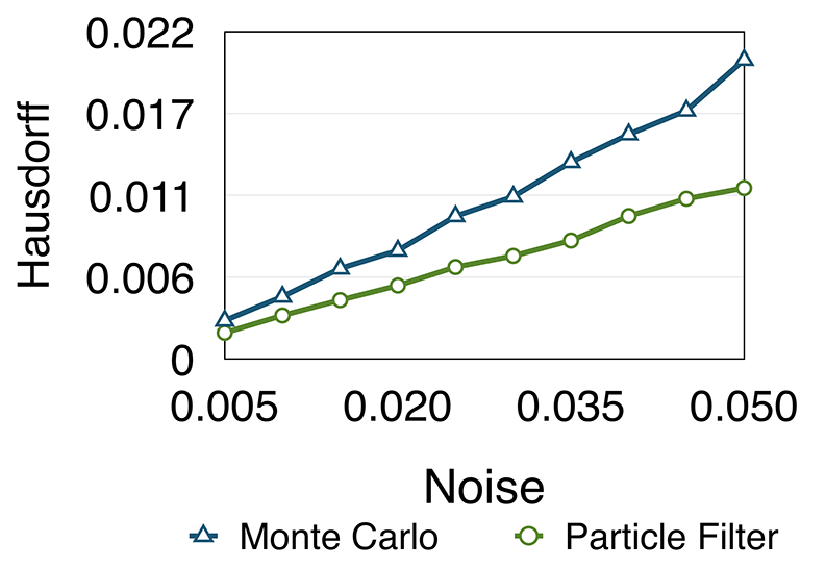
\includegraphics[height=1.0in]{../figures/doublegyre_h.eps}
    \caption{}
  \end{subfigure}~
  \begin{subfigure}[b]{0.24\textwidth}
    \centering
    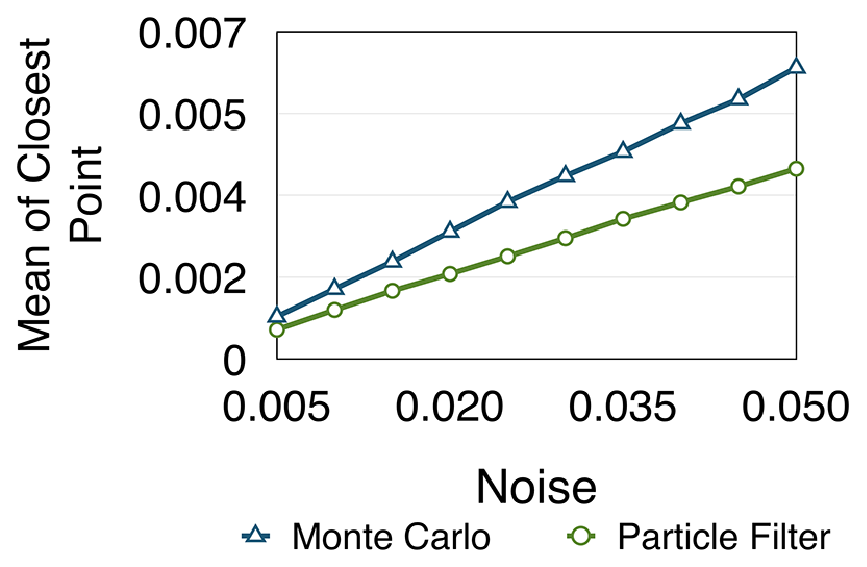
\includegraphics[height=1.0in]{../figures/doublegyre_m.eps}
    \caption{}
  \end{subfigure}
  \caption{Comparison of the distance between the most likely traces and the ground truth using Hausdorff and mean of the closest point measurements for our method and the MC method.}
  \label{gerror}
\end{figure}

\begin{figure}[!htb]
  \centering
  \begin{subfigure}[b]{0.24\textwidth}
    \centering
    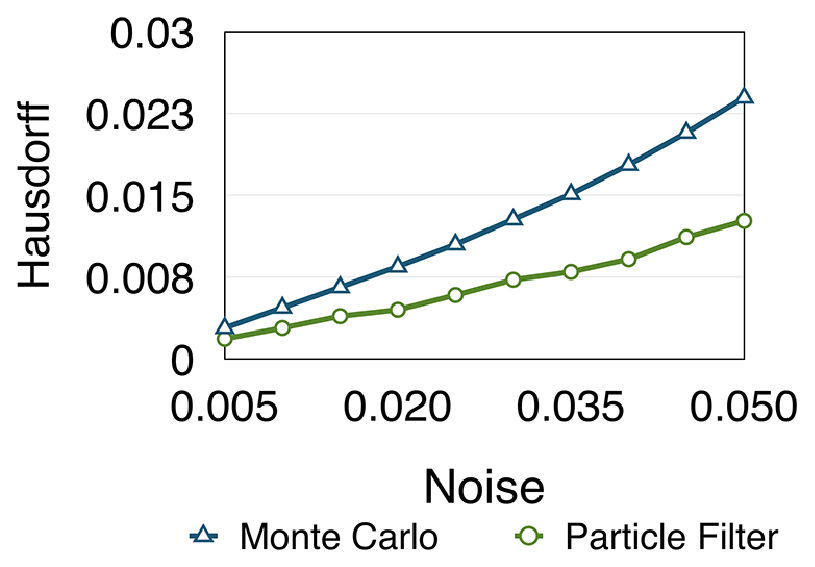
\includegraphics[height=1.0in]{../figures/doublegyre_hr.eps}
    \caption{}
  \end{subfigure}~
  \begin{subfigure}[b]{0.24\textwidth}
    \centering
    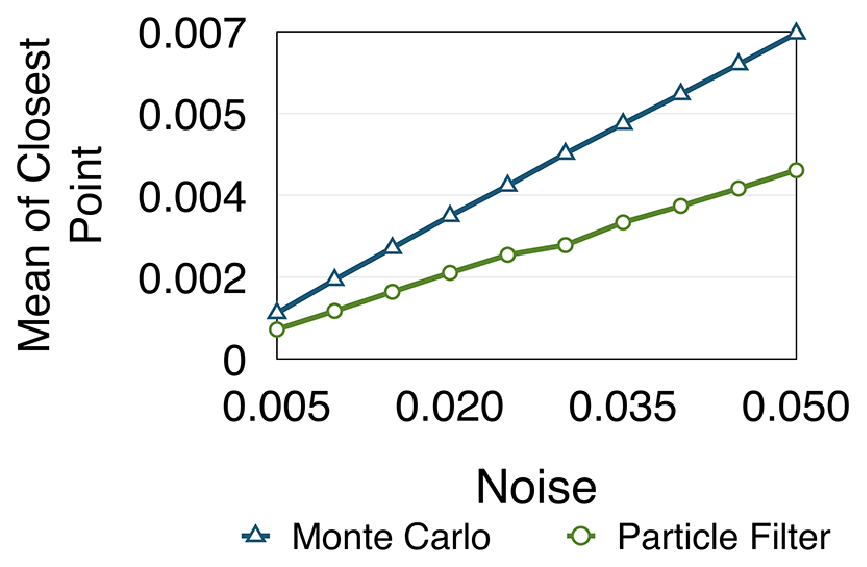
\includegraphics[height=1.0in]{../figures/doublegyre_mr.eps}
    \caption{}
  \end{subfigure}
  \caption{Comparison of overall trace accuracy. For each method, distances of all sample traces to the ground truth are measured and summed by their weights.}
  \label{gerror_r}
\end{figure}

Figure~\ref{case_1} shows sample traces generated by the MC method and the proposed method at a given seed location in the double-gyre flow field. As we can see in the figure, our method can generate more concentrated traces which are also closer to the ground truth compared with the MC method. The most likely trace generated by the proposed method is also closer to the ground truth, as shown in~\ref{case_1_c}.

\begin{figure}[!htb]
  \centering
  \begin{subfigure}[!htb]{0.25\textwidth}
    \centering
    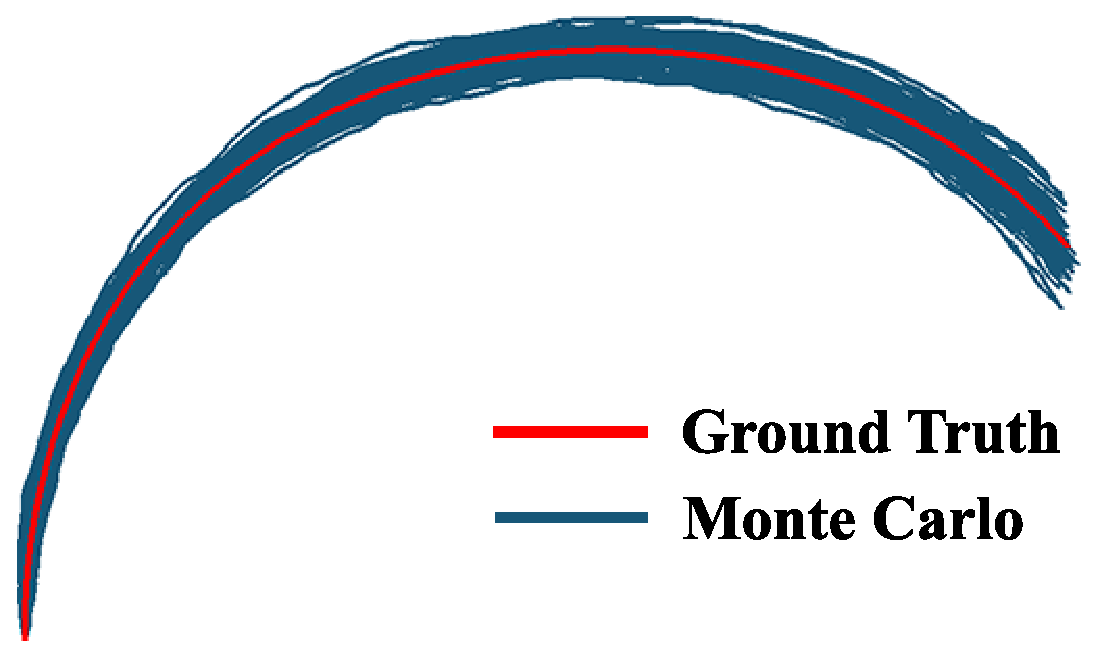
\includegraphics[height=0.8in]{../figures/double_gyre_mc35.eps}
    \caption{}
    \label{case_1_a}
  \end{subfigure}~
  \begin{subfigure}[!htb]{0.25\textwidth}
    \centering
    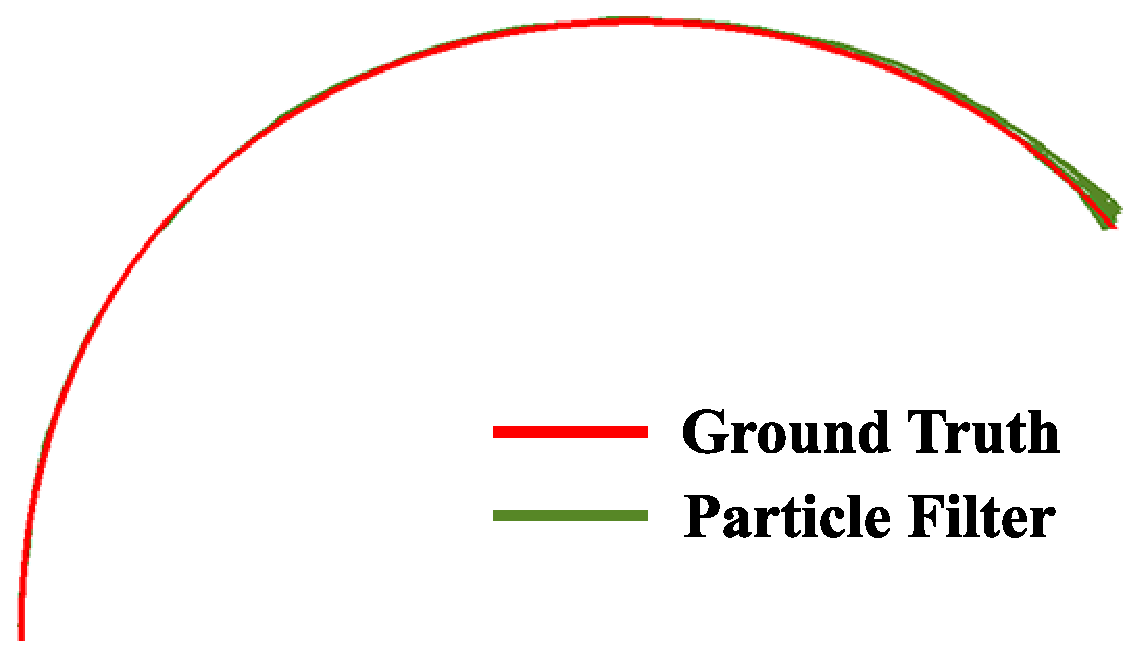
\includegraphics[height=0.8in]{../figures/double_gyre_smc35.eps}
    \caption{}
    \label{case_1_b}
  \end{subfigure}

  \begin{subfigure}[!htb]{0.5\textwidth}
    \centering
    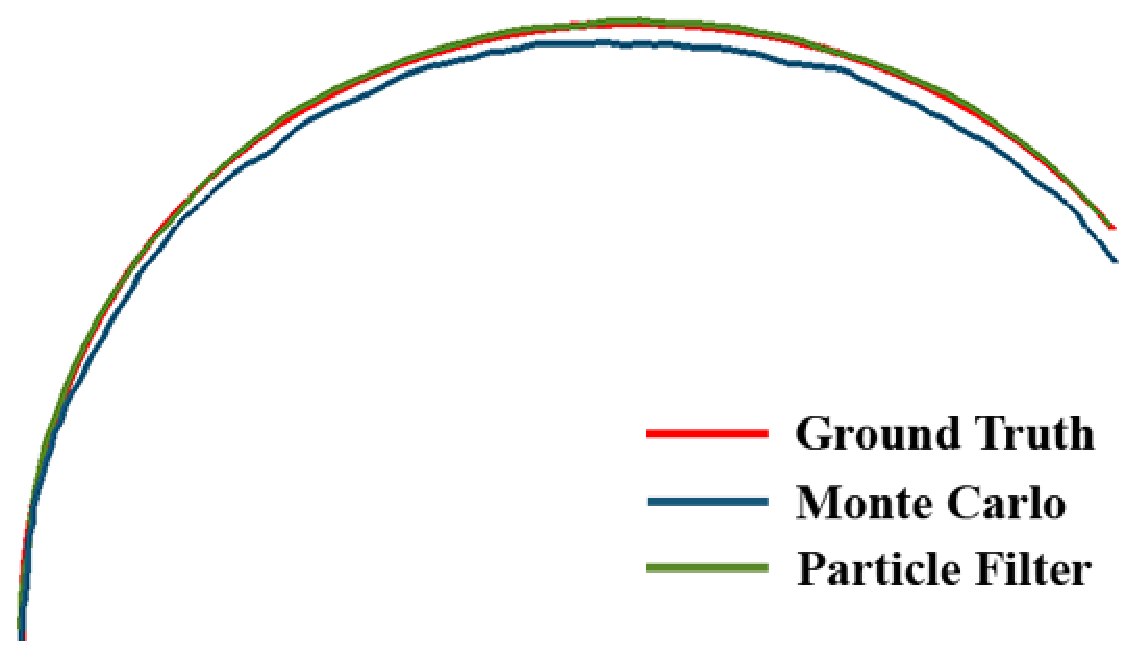
\includegraphics[height=1.0in]{../figures/double_gyre_opt35.eps}
    \caption{}
    \label{case_1_c}
  \end{subfigure}
  \caption{(a): Sampled streamlines computed by the MC method starting from seeding position $x=0.3, y=0.5$ in the analytical double-gyre data set. (b): Sampled streamlines computed by our method from the same seeding position in (a). (c): The most likely traces generated by both methods compared with the ground truth.}
  \label{case_1}
\end{figure}

\subsection{Spatially aggregated Data Sets}

In this section, experiments were done on two real-world flow field data sets, including Hurricane Isabel and 2D Ocean. Hurricane Isabel is a data set with a resolution of $500 \times 500 \times 100$ that models a strong hurricane in the west Atlantic region in September 2003. The 2D Ocean data set is a flow data with a resolution of $574 \times 289$ produced by a 2D computational fluid dynamics simulation. In order to test the performance of our algorithm on uncertain data which represented by non-gaussian distributions, we decompose the data into small cubic blocks and construct a histogram for each block. To compute a histogram from a set of vector directions, we consider the surface patches of a unit sphere as histogram bins. We make use of the recursive zonal equal area sphere partitioning algorithm~\cite{leopardi2006} to partition the unit sphere into patches of equal area and use them as our histograms bins. Partition results for different number of patches on the $2$-dimensional unit sphere are shown in Figure~\ref{rzeasp}. In the experiments, we partition the sphere into $2048$ patches to make an accurate histogram. As Carr et at. presented in~\cite{Carr:2006:HIS:1187627.1187777}, histograms can be poor representations of data since they represent the distribution using the nearest neighbor interpolation. To address this issue, we densely sample the data in each local block to make the histogram converge to the true local distribution. For the test data sets, distribution-based data are generated with three different block size $8^3$, $16^3$, and $32^3$ to evaluate the performance of the proposed algorithm under the influence of uncertainty.

Since the data are represented as block-wise histograms, how to interpolate between neighboring blocks to generate a more accurate probability distribution becomes a challenging question. Developing efficient and accurate interpolation technique from probability density functions is still an active area for research. A variety of techniques~\cite{10.1109/TVCG.2013.208, 10.1109/TVCG.2012.249} have been proposed to perform linear interpolation on different types of distributions. However, they are only focused on either uniform or parametric distributions. Furthermore, these techniques can only work on point based data sets. They may give incorrect value ranges for block-based data sets used in the experiments. Here, we perform the interpolation by aggregating the contributions of neighboring histograms to the distribution of interest based on the method presented by Clemen et al. in~\cite{aggregation99}
\begin{equation}
  {h(\theta)} = k\prod\limits_{i = 1}^n {h{{_i}(\theta)}^{{\alpha _i}}}
\end{equation}
where $k$ is a normalizing constant and the weights ${{\alpha _i}}$ represent the relative quality of the different histograms. Typically, the weights are restricted to sum to one. The contribution of each histogram is estimated by applying convolution operations on it with a von Mises-Fisher kernel, where the number of the convolution operations is determined based on the distance between the neighboring block and target position.

\begin{figure}[htb!f]
  \centering
  \begin{subfigure}[b]{0.16\textwidth}
    \centering
    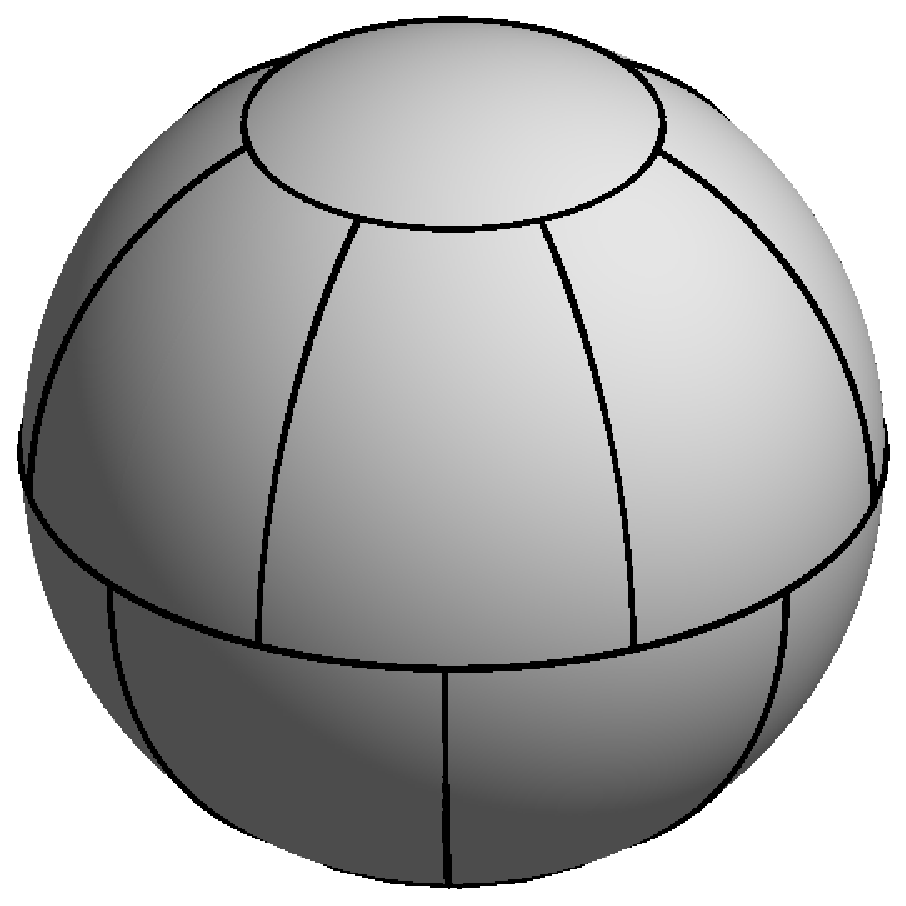
\includegraphics[width=0.8in]{../figures/rzeasp_16.eps}
    \caption{16 patches}
  \end{subfigure}~
  \begin{subfigure}[b]{0.16\textwidth}
    \centering
    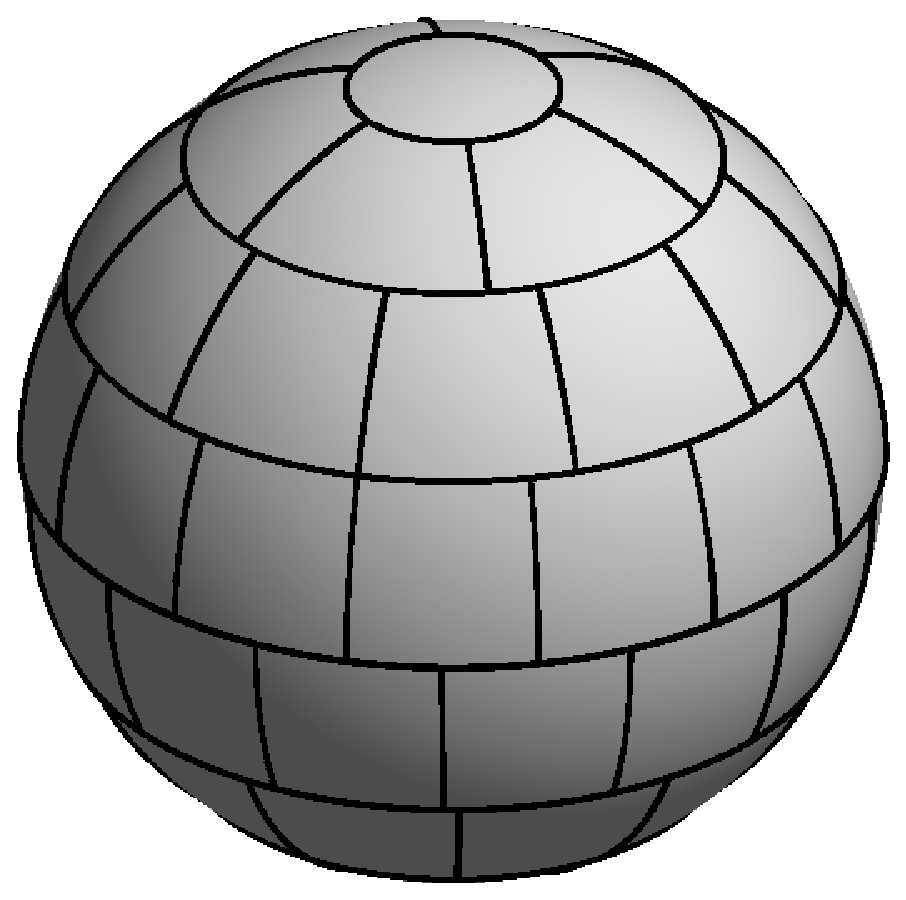
\includegraphics[width=0.8in]{../figures/rzeasp_64.eps}
    \caption{64 patches}
  \end{subfigure}~
  \begin{subfigure}[b]{0.16\textwidth}
    \centering
    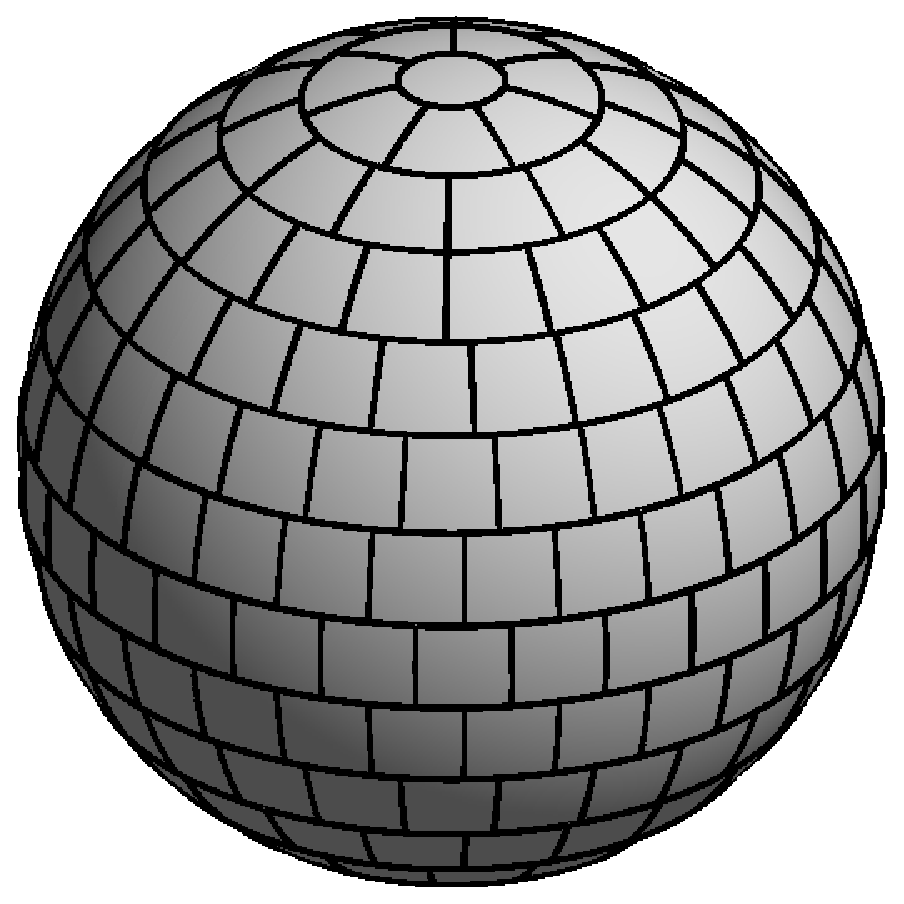
\includegraphics[width=0.8in]{../figures/rzeasp_256.eps}
    \caption{256 patches}
  \end{subfigure}
  \caption{Recursive zonal equal area sphere partitioning with different number of patches.}
  \label{rzeasp}
\end{figure}

As presented above, we regularly sample a set of seed locations and compute the streamlines for both the raw data and the spatially down sampled data. The sample seed positions and the number of samples for the two test data sets are given in Table~\ref{seed_position}. To perform the quantitative analysis, we treat the streamlines computed from the raw data as the ground truth and compute the distance between the stochastic particle traces with the ground truth. $100$ particles were used with a integration step size $1.0$ and a maximum step number of $1000$ for the streamline computation. For the particle filtering method, a concentration parameter $\kappa = 60$ and a resampling threshold $N_t = 4.0$ are used. Figure~\ref{berror_r} gives the mean of the distances' weighted sum between sample streamline bundles generated from the test methods and the ground truth on different data sets with different block sizes. The figure reveals that the proposed method can produce traces that are closer to the ground truth.

\begin{table}[ht!b]
\centering
\begin{tabular}{|l|l|l|}
\hline
Data Set & Number of Seeds                 & Interval of Seed Positions  \\ \hline
Isabel   & $12 \times 12 \times 9$ (1296)  & $40 \times 40 \times 10$    \\ \hline
Ocean    & $28 \times 14$ (392)            & $20 \times 20$              \\ \hline
\end{tabular}
\caption{Sample seed positions for the two test data sets.}
\label{seed_position}
\end{table}

% \begin{figure}[!htb]
%   \centering
%   \begin{subfigure}[b]{0.24\textwidth}
%     \centering
%     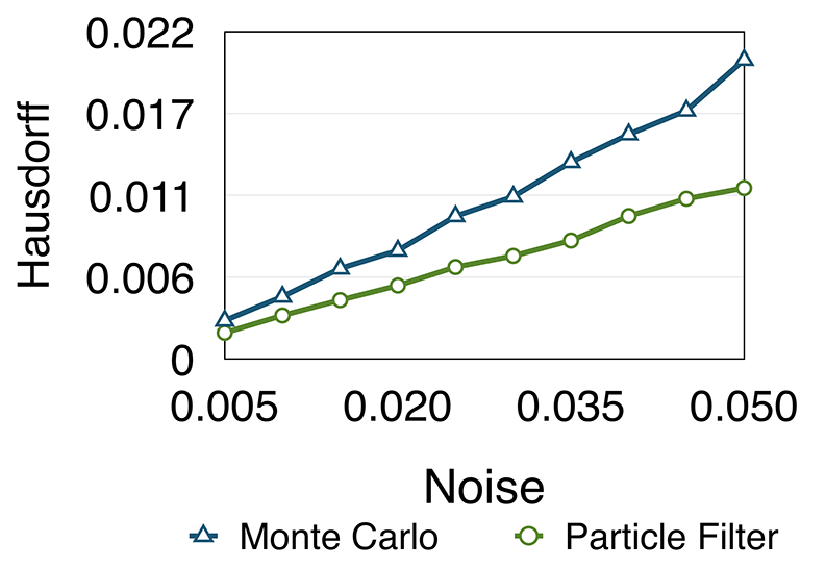
\includegraphics[height=0.9in]{../figures/doublegyre_h.eps}
%     \caption{}
%   \end{subfigure}~
%   \begin{subfigure}[b]{0.24\textwidth}
%     \centering
%     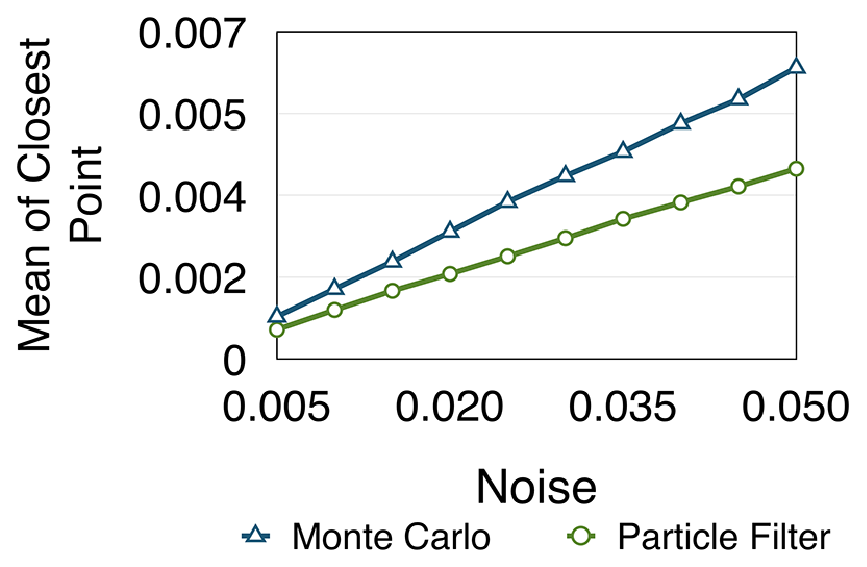
\includegraphics[height=0.9in]{../figures/doublegyre_m.eps}
%     \caption{}
%   \end{subfigure}

%   \begin{subfigure}[b]{0.24\textwidth}
%     \centering
%     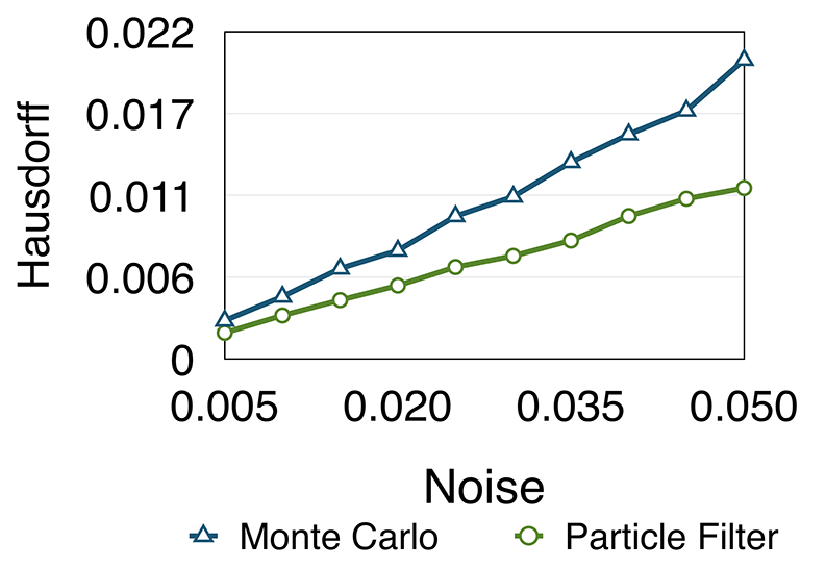
\includegraphics[height=0.9in]{../figures/doublegyre_h.eps}
%     \caption{}
%   \end{subfigure}~
%   \begin{subfigure}[b]{0.24\textwidth}
%     \centering
%     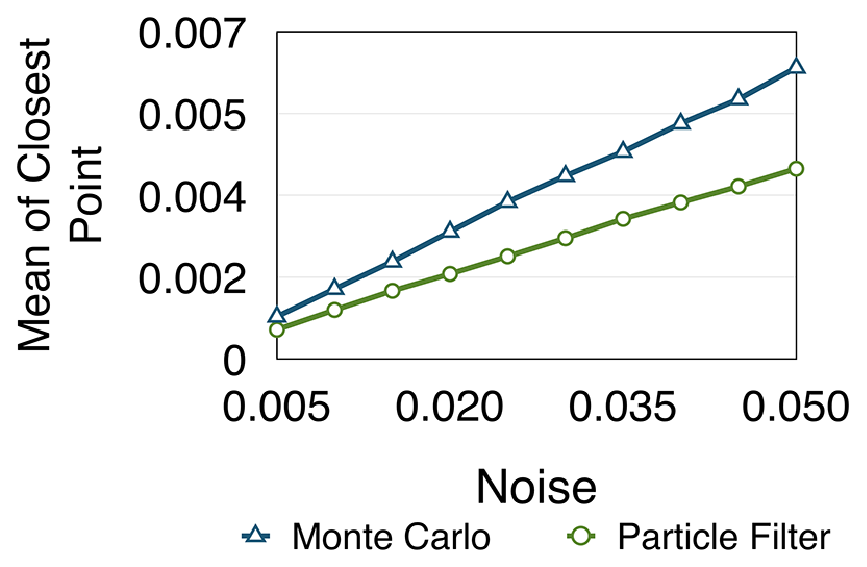
\includegraphics[height=0.9in]{../figures/doublegyre_m.eps}
%     \caption{}
%   \end{subfigure}
%   \caption{Hausdorff and mean of the closest point distances between the ground truth and most likely traces generated by our method and the MC method for the two spacial down-sampled data sets.}
%   \label{berror}
% \end{figure}

\begin{figure}[!htb]
  \centering
  \begin{subfigure}[b]{0.24\textwidth}
    \centering
    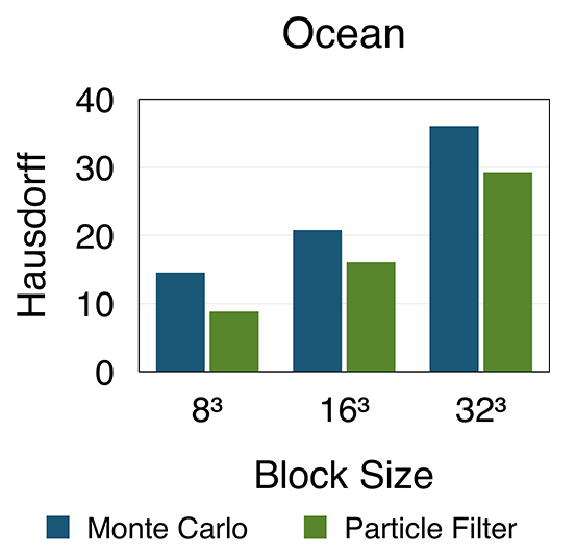
\includegraphics[height=1.0in]{../figures/ocean_h.eps}
    \caption{}
  \end{subfigure}~
  \begin{subfigure}[b]{0.24\textwidth}
    \centering
    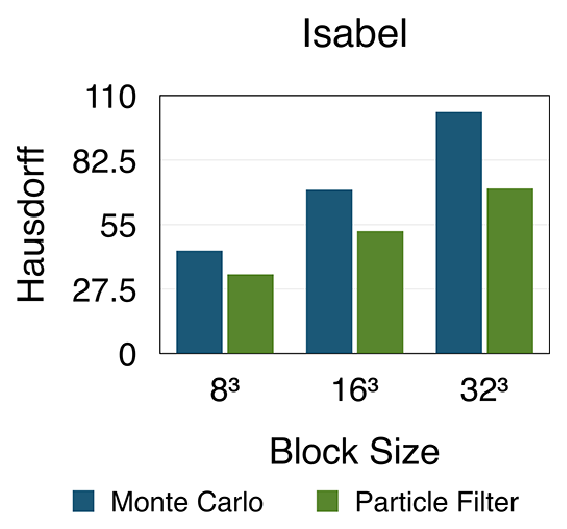
\includegraphics[height=1.0in]{../figures/isabel_h.eps}
    \caption{}
  \end{subfigure}

  \begin{subfigure}[b]{0.24\textwidth}
    \centering
    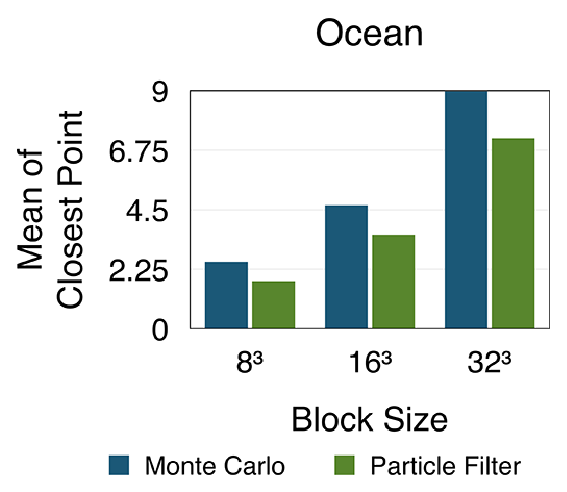
\includegraphics[height=1.0in]{../figures/ocean_m.eps}
    \caption{}
  \end{subfigure}~
  \begin{subfigure}[b]{0.24\textwidth}
    \centering
    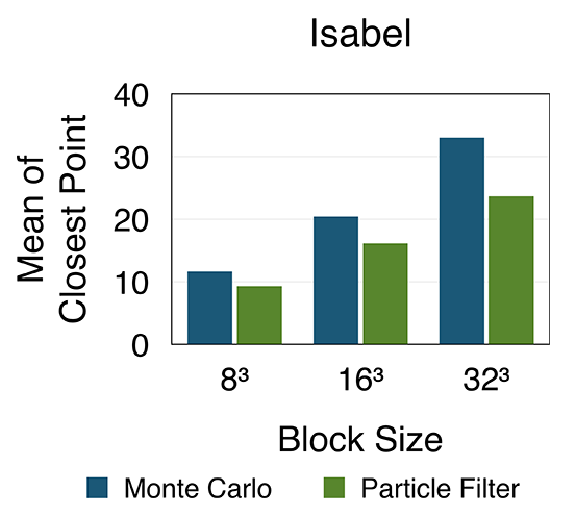
\includegraphics[height=1.0in]{../figures/isabel_m.eps}
    \caption{}
  \end{subfigure}
  \caption{Hausdorff and mean of the closest point distances between the ground truth and sample traces generated by our method and the MC method for the two spatially aggregated data sets.}
  \label{berror_r}
\end{figure}

Figure~\ref{data_overview} shows the streamlines generated from the two test data sets on the seed positions presented above. In Figure~\ref{data_overview} (a) and (d), the ground truth streamlines are generated from the raw data. The most likely streamlines generated by the MC method on the distribution-based data set with block size $16^3$ are given in Figure~\ref{data_overview} (b) and (e); as expected, streamlines generated by the MC method are generally not as smooth as the ground truth and some flow features looks quiet different compare with the ground truth. Figure~\ref{data_overview} (c) and (f) show the streamlines produced by our method with the same block size, which give more accurate and smoother results. In addition to the most likely traces, the distribution approximated by the estimated sample traces is also important for understanding the distribution-based flow field. The visualization of the estimated streamline bundles on different flow field data sets are shown in Figure~\ref{case_5} and~\ref{case_4} to demonstrate the advantage of the proposed method. The resulting trajectories are generated with $1000$ particles for the Monte Carlo method and the particle filtering algorithm. By considering the correlation of vector directions in the spacial domain, our method is less sensitive to the local uncertainty, when MC traces can scatter to wrong directions, as show in ~\ref{case_5}. Figure~\ref{case_4} shows that our algorithm can produce more concentrated results than the basic MC method, because the correlation between consecutive integration steps (the prior information) are exploited.

\begin{figure*}[!htb]
  \centering
  \begin{subfigure}[!htb]{0.32\textwidth}
    \centering
    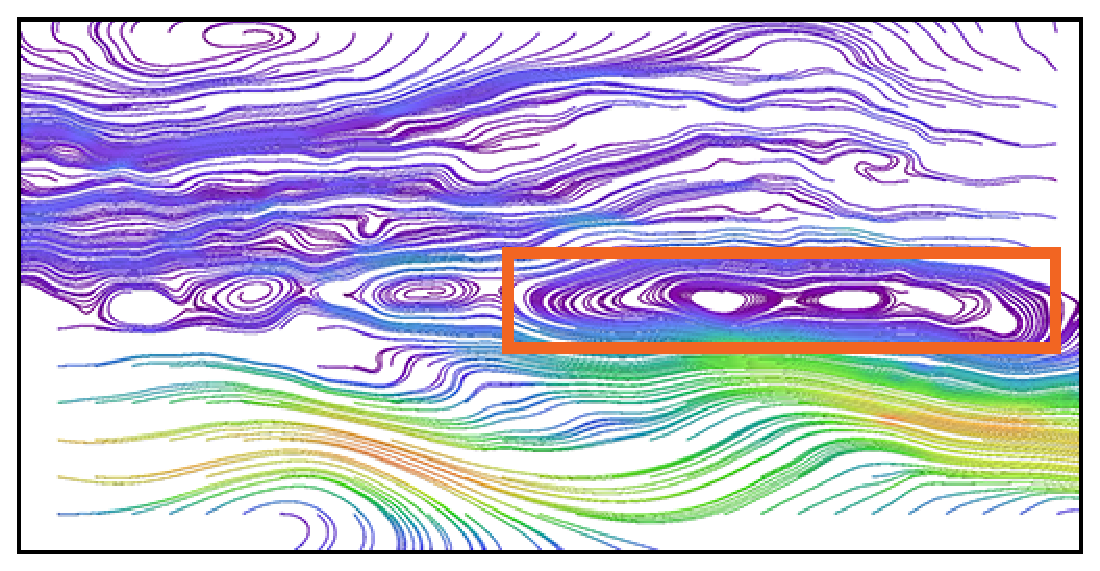
\includegraphics[width=2.2in]{../figures/ocean_gt.eps}
    \caption{}
  \end{subfigure}~
  \begin{subfigure}[!htb]{0.32\textwidth}
    \centering
    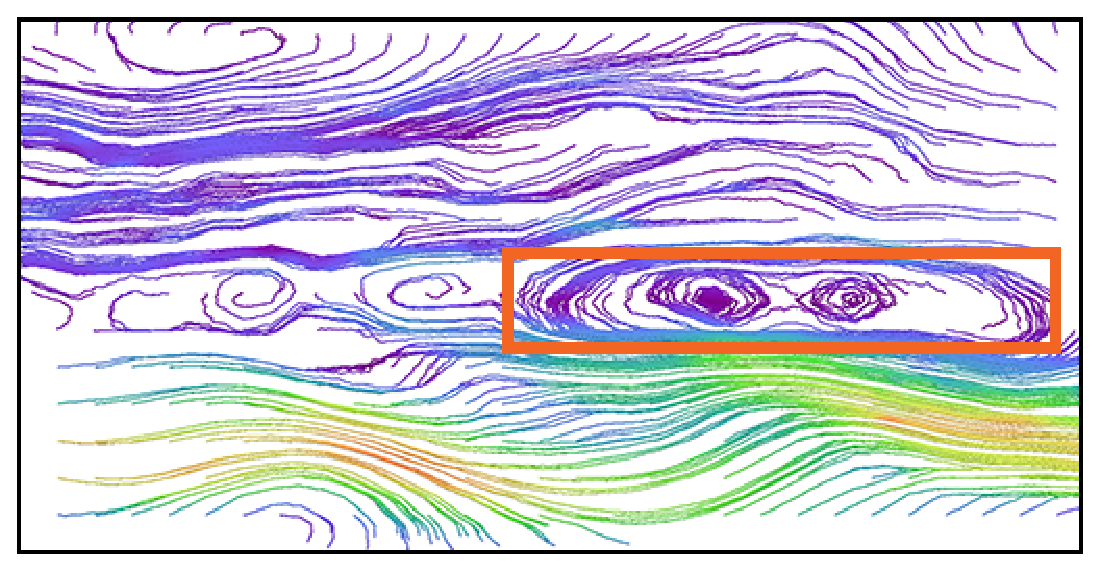
\includegraphics[width=2.2in]{../figures/ocean_mc.eps}
    \caption{}
  \end{subfigure}~
  \begin{subfigure}[!htb]{0.32\textwidth}
    \centering
    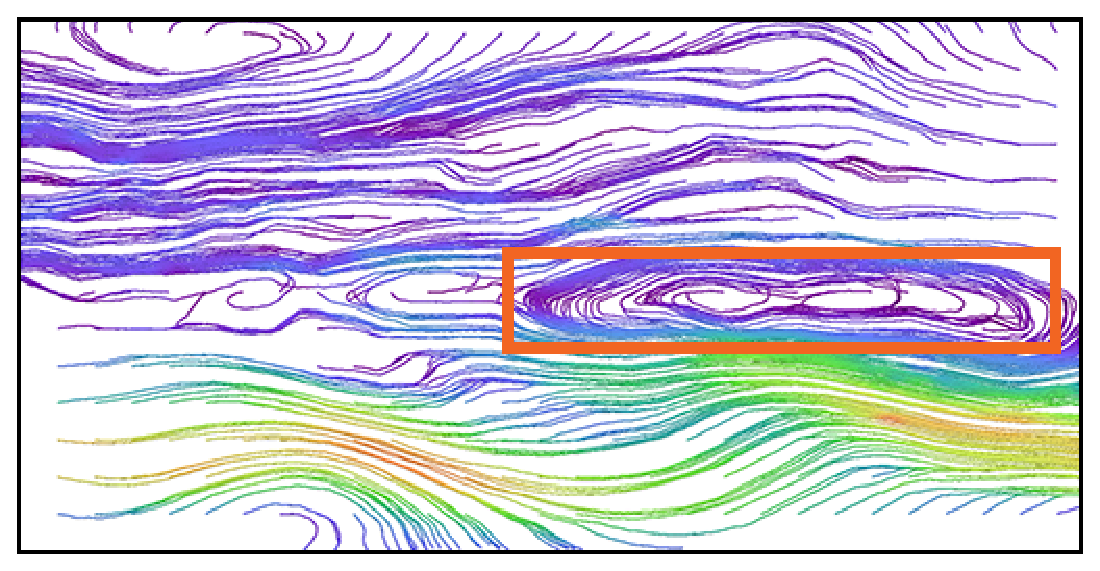
\includegraphics[width=2.2in]{../figures/ocean_smc.eps}
    \caption{}
  \end{subfigure}

  \begin{subfigure}[!htb]{0.32\textwidth}
    \centering
    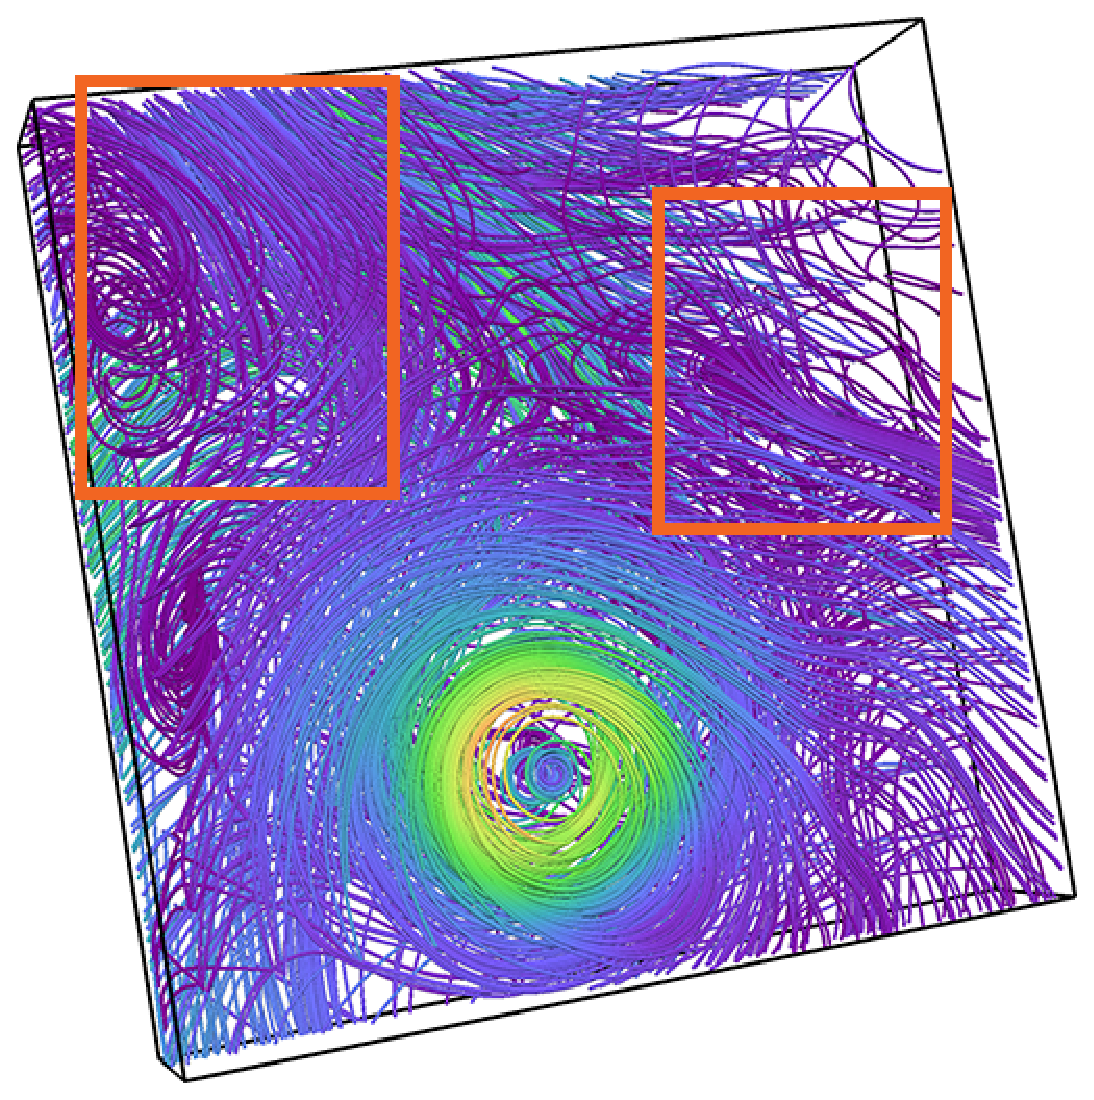
\includegraphics[width=2.2in]{../figures/isabel_gt.eps}
    \caption{}
  \end{subfigure}~
  \begin{subfigure}[!htb]{0.32\textwidth}
    \centering
    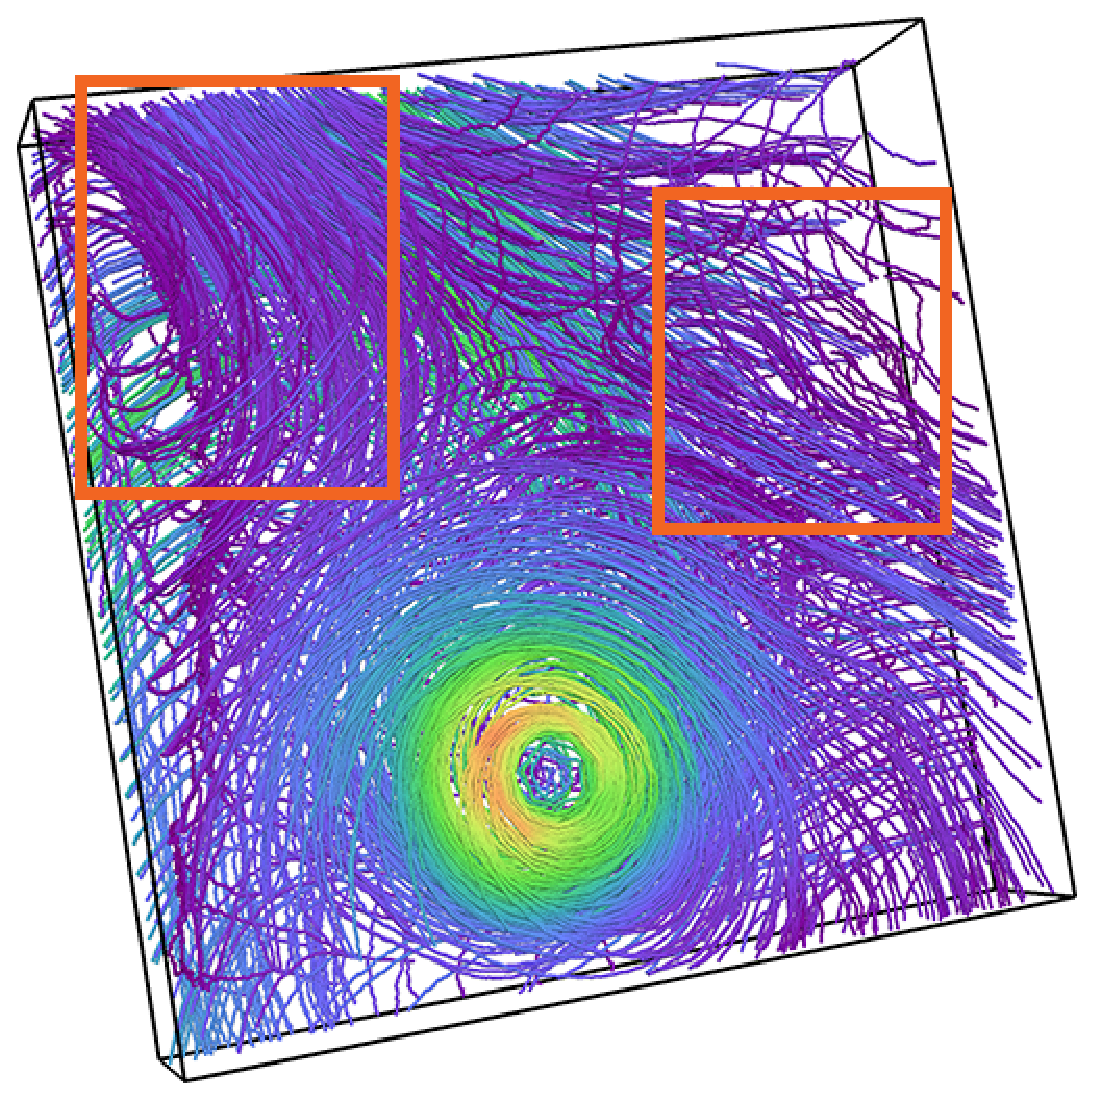
\includegraphics[width=2.2in]{../figures/isabel_mc.eps}
    \caption{}
  \end{subfigure}~
  \begin{subfigure}[!htb]{0.32\textwidth}
    \centering
    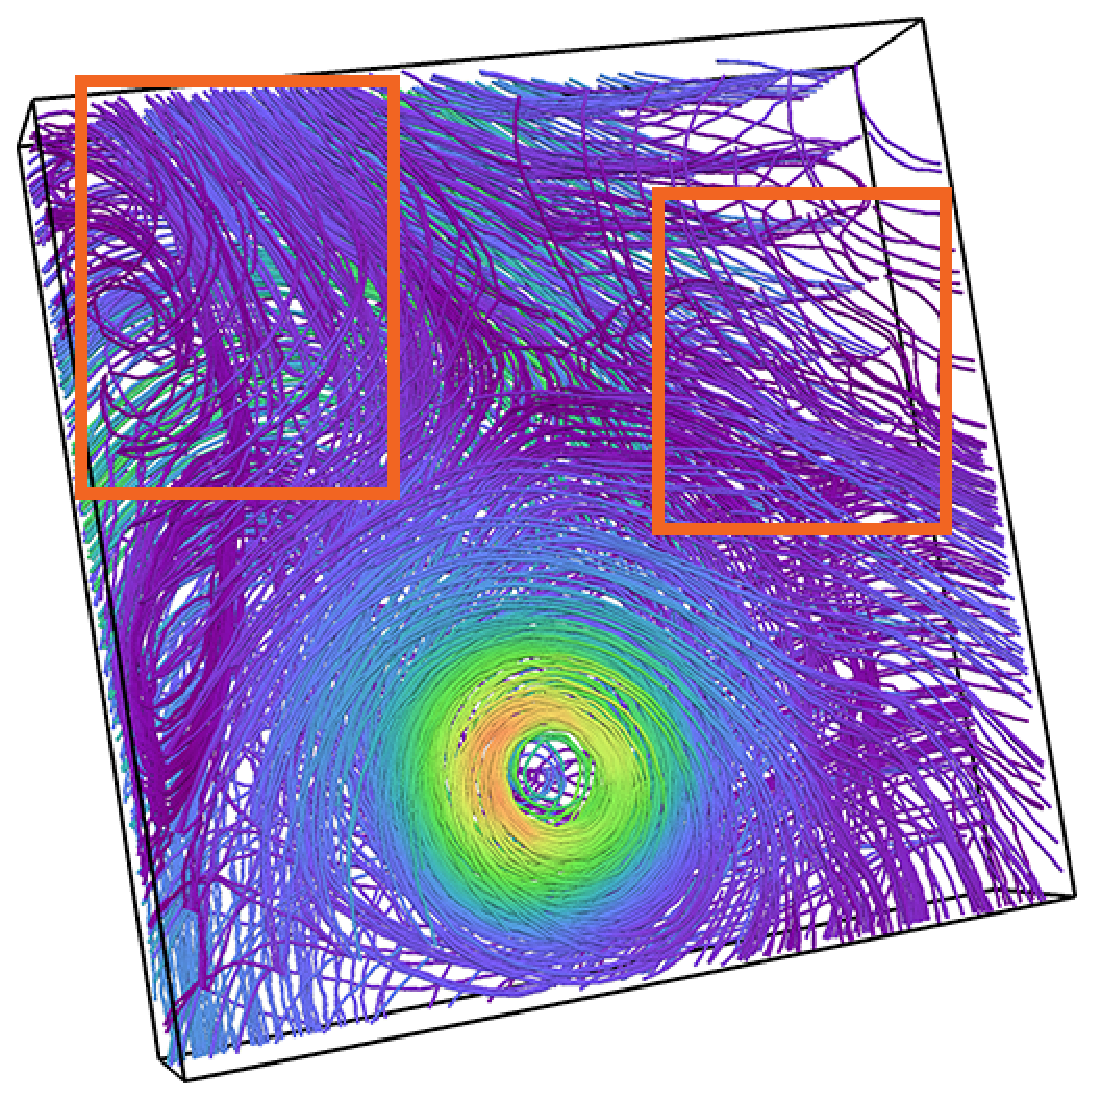
\includegraphics[width=2.2in]{../figures/isabel_smc.eps}
    \caption{}
  \end{subfigure}

  \caption{Streamlines generated on the 2D Ocean and the Hurricane Isabel data sets. The color is used to enhance the contrast among streamlines. (a) and (d): The ground truth streamlines generated on the raw data. (b) and (e): Results produced by the Monte Carlo method on the distribution data with block size $16^3$, introduce noisy patterns on the streamlines due to the local uncertainty and give inaccurate overview of the flow features. Our particle filter method gives more accurate overview results and smoother streamlines by exploiting the spatial coherence of the vector directions, shown in (c) and (f).}
  \label{data_overview}
\end{figure*}

\begin{figure}[!htb]
  \centering
  \begin{subfigure}[!htb]{0.5\textwidth}
    \centering
    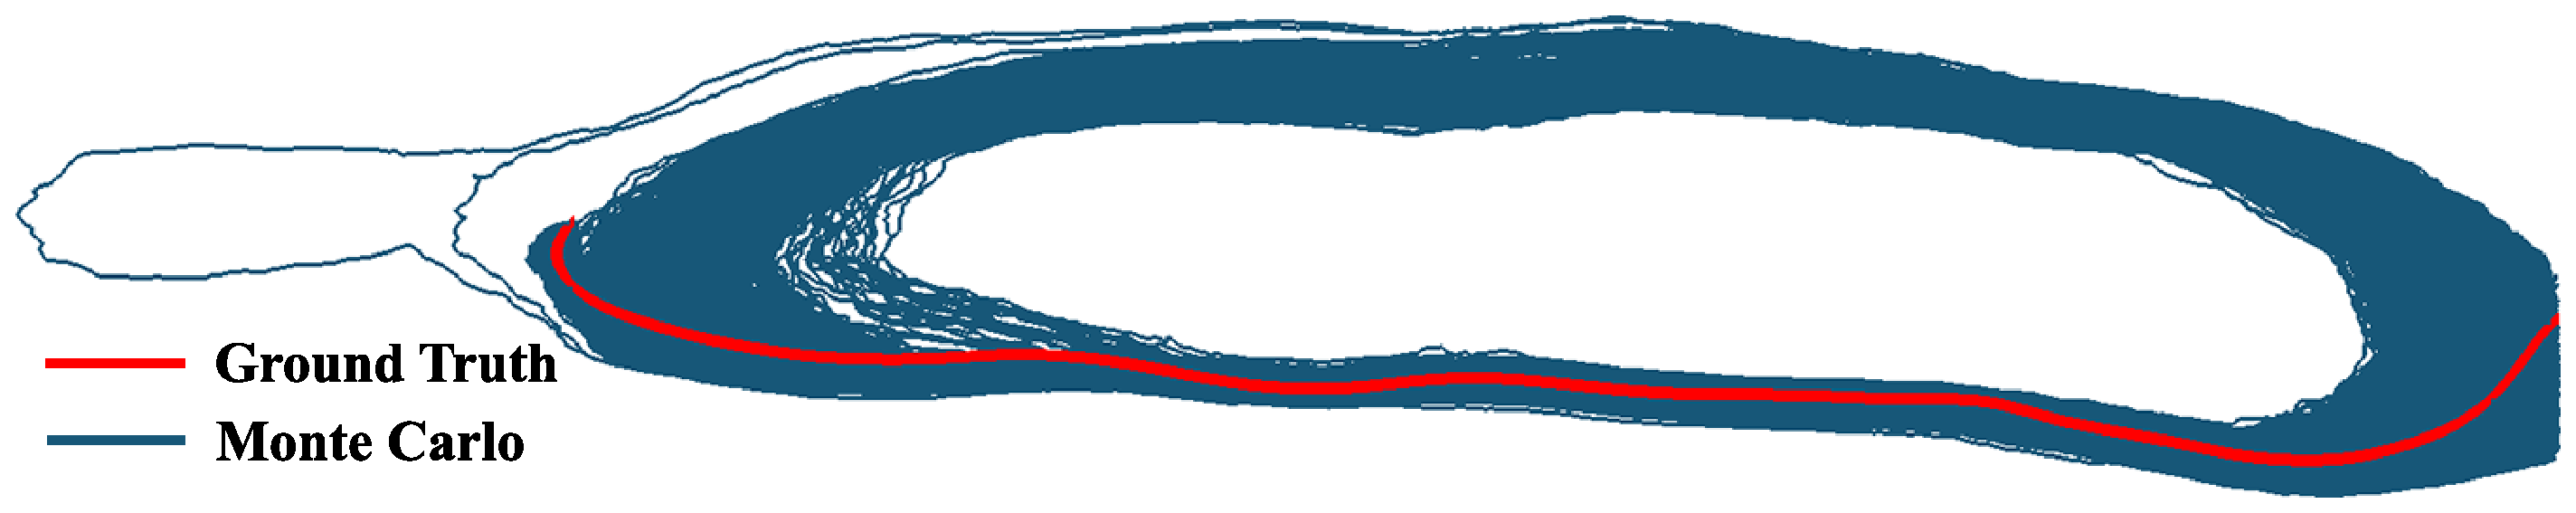
\includegraphics[width=2.8in]{../figures/ocean_mc1.eps}
    \caption{}
    \label{case_5_a}
  \end{subfigure}

  \begin{subfigure}[!htb]{0.5\textwidth}
    \centering
    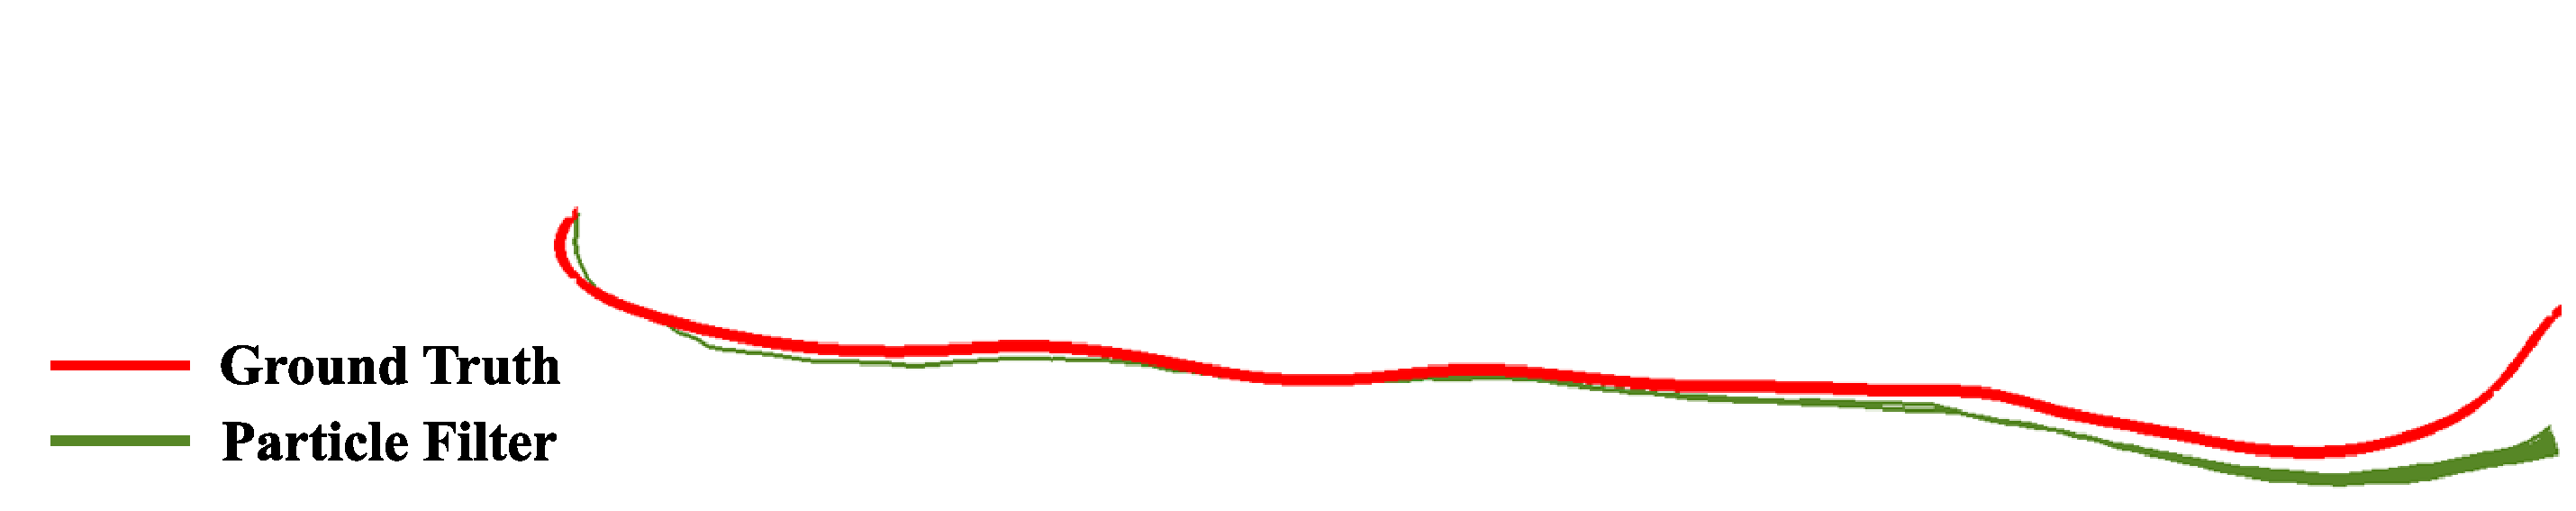
\includegraphics[width=2.8in]{../figures/ocean_smc1.eps}
    \caption{}
    \label{case_5_b}
  \end{subfigure}
  \caption{(a): Sampled streamlines computed by the MC method starting from seeding position $x=280, y=140$ in the 2D Ocean data set. (b): Sampled streamlines computed by our method from the same seeding position in (a).}
  \label{case_5}
\end{figure}

\begin{figure}[!htb]
  \centering
  \begin{subfigure}[!htb]{0.25\textwidth}
    \centering
    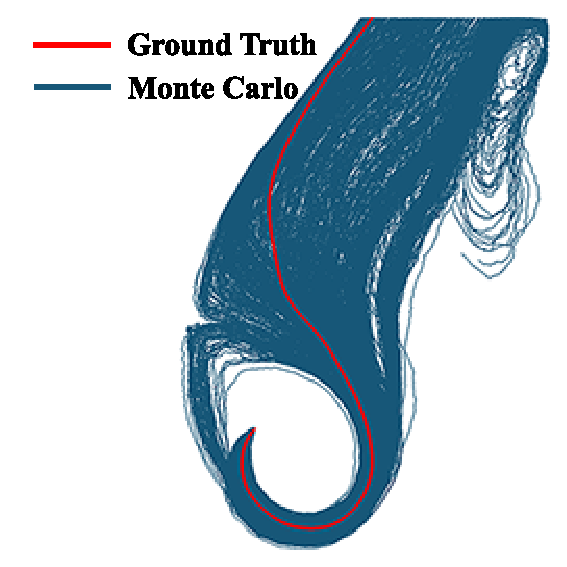
\includegraphics[height=1.4in]{../figures/isabel_mc1.eps}
    \caption{}
    \label{case_4_a}
  \end{subfigure}~
  \begin{subfigure}[!htb]{0.25\textwidth}
    \centering
    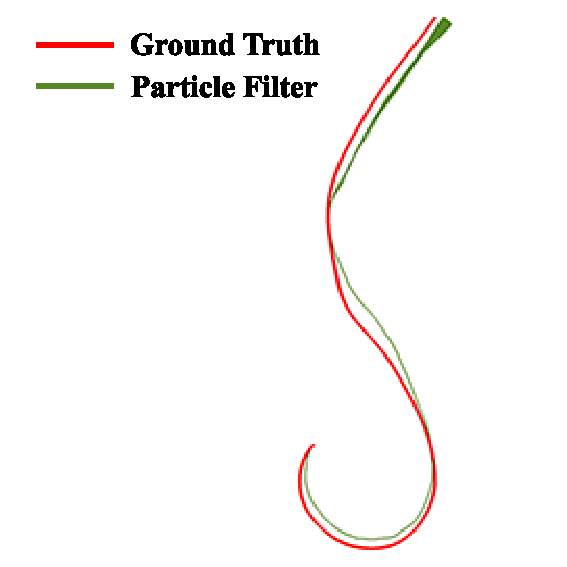
\includegraphics[height=1.4in]{../figures/isabel_smc1.eps}
    \caption{}
    \label{case_4_b}
  \end{subfigure}
  \caption{(a): Sampled streamlines computed by the MC method starting from seeding position $x=250, y=150, z=45$ in the Isabel data set. (b): Sampled streamlines computed by our method from the same seeding position in (a).}
  \label{case_4}
\end{figure}

\subsection{Performance}

All the experiments were performed on a desktop computer with an Intel(R) Core(TM) i7-4790K CPU 4.0GHz processor, 16GB memory, and an NVIDIA GTX 970 GPU. In Table~\ref{timing}, we compare the performance measurements between the particle filtering algorithm and the Monte Carlo method for streamlines estimated for a given seed position with $100$ sample points for all the test data sets used in this paper. In all the datasets, our approach is almost as fast as the Monte Carlo algorithm.

\begin{table}[!htb]
\centering
\begin{tabular}{|c|c|c|c|c|}
\hline
\multirow{2}{*}{Data Set}    & \multirow{2}{*}{Method}     & \multicolumn{3}{c|}{Timing(sec)}  \\ \cline{3-5}
                             &                             & 40 Steps  & 80 Steps & 120 Steps  \\ \hline
\multirow{2}{*}{Double Gyre} & MC                          & 0.0026    & 0.005    & 0.008      \\ \cline{2-5}
                             & Particle Filter             & 0.0035    & 0.007    & 0.01       \\ \hline
\multirow{2}{*}{Ocean 2D}    & MC                          & 2.8       & 5.9      & 9.1        \\ \cline{2-5}
                             & Particle Filter             & 2.9       & 6.1      & 9.3        \\ \hline
\multirow{2}{*}{Isabel}      & MC                          & 3.3       & 6.7      & 10.1       \\ \cline{2-5}
                             & Particle Filter             & 3.4       & 6.8      & 10.7       \\ \hline

\end{tabular}
\caption{Overview of the performance for the particle filtering algorithm and the Monte Carlo method tested on all the distribution-based data sets used in this paper.}
\label{timing}
\end{table}
